% !TEX root = ../entropy.tex

\section{Results}%
\label{sec:results}

\subsection{New results}%
\label{sub:new_results}

\foreach \endog in {has_sa_inflows,sa_inflows,sa_netflows,sa_outflows} {
    \foreach \cat in {tag,tag_auto,merchant,groc} {
        \input{\tabdir/reg_\endog_\cat.tex}}}


\subsection{Effect of entropy on saving}%
\label{sub:effect_of_entropy_on_saving}

Entropy measures are calculated based on the probability of occurrence of a
pattern within a user month. Implicitly, this assumes that move diverse
spending reflects more chaotic behaviour. The outcome variable is a dummy
indicating whether a user made at least one transfer into their savings account
in a given month.

\begin{itemize}

    \item Table~\ref{tab:reg_entropy_savings_fe} shows results with a full set
        of controls for different FE specifications.
        Table~\ref{tab:reg_entropy_savings_obo} summarises shows controls added
        cumulatively.

    \item For smoothed entropy, the results are as hypothesised: higher entropy
        is strongly and robustly associated with a lower probability of making
        a savings transaction.

    \item Curiously, though, unsmoothed entropy is even more strongly but
        positively related to making a savings transaction.

    \item Figure~\ref{fig:entropy_tag_vs_nunique} shows that smoothing
        increases entropy scores for those profiles with txns in few unique
        categories (the reason is that a low number of unique categories
        implies a high number of categories with zero counts, and smoothing
        reverses the implication of zero counts from 'zero entropy' to 'max
        entropy').

    \item Smoothed entropy is high when the number of unique categories is low
        (and zero categories high), and it is negatively related to saving.
        Hence: user-months with spends across few categories are less likely to
        save.

        Unsmoothed entropy is high when spends across categories are equal and
        the total number of spends is high.

\end{itemize}


\begin{table}[htbp]
   \centering
   \footnotesize
   \begin{threeparttable}[b]
      \caption{\label{tab:reg_entropy_savings_fe} FE specifications}
      \begin{tabular}{lccc}
         \tabularnewline \midrule \midrule
         Dependent Variable: & \multicolumn{3}{c}{has\_sa\_inflows}\\
         Model:              & (1)              & (2)              & (3)\\  
         \midrule
         \emph{Variables}\\
         entropy\_tag\_sz    & -0.051$^{***}$   & -0.059$^{***}$   & -0.047$^{***}$\\   
                             & [-0.058; -0.043] & [-0.072; -0.046] & [-0.060; -0.034]\\   
         entropy\_tag\_z     & 0.104$^{***}$    & 0.105$^{***}$    & 0.081$^{***}$\\   
                             & [0.092; 0.116]   & [0.084; 0.125]   & [0.060; 0.102]\\   
         Regular savings     & 0.581$^{***}$    & 0.202$^{***}$    & 0.196$^{***}$\\   
                             & [0.573; 0.589]   & [0.186; 0.217]   & [0.180; 0.212]\\   
         Credit spend        & -0.141$^{***}$   & -0.052$^{***}$   & -0.052$^{***}$\\   
                             & [-0.156; -0.126] & [-0.087; -0.017] & [-0.087; -0.017]\\   
         Month spend         & 0.009$^{***}$    & 0.019$^{***}$    & 0.019$^{***}$\\   
                             & [0.008; 0.011]   & [0.017; 0.022]   & [0.016; 0.021]\\   
         Urban               & 0.006            & 0.010            & -0.002\\   
                             & [-0.002; 0.015]  & [-0.178; 0.199]  & [-0.189; 0.186]\\   
         Month income        & -0.018$^{***}$   & 0.007$^{*}$      & 0.005\\   
                             & [-0.020; -0.016] & [-0.0004; 0.014] & [-0.002; 0.012]\\   
         Has income in month & 0.089$^{***}$    & 0.038$^{***}$    & 0.035$^{**}$\\   
                             & [0.067; 0.112]   & [0.011; 0.066]   & [0.007; 0.063]\\   
         Loan repayment      & -0.010$^{***}$   & 0.001            & 0.0005\\   
                             & [-0.016; -0.003] & [-0.014; 0.017]  & [-0.015; 0.016]\\   
         (Intercept)         & 0.232$^{***}$    &                  &   \\   
                             & [0.208; 0.256]   &                  &   \\   
         \midrule
         \emph{Fixed-effects}\\
         User id             &                  & Yes              & Yes\\  
         Calendar month      &                  &                  & Yes\\  
         \midrule
         \emph{Fit statistics}\\
         Observations        & 89,169           & 89,169           & 89,169\\  
         R$^2$               & 0.19330          & 0.42488          & 0.42727\\  
         Within R$^2$        &                  & 0.03210          & 0.02647\\  
         \midrule \midrule
         \multicolumn{4}{l}{\emph{Signif. Codes: ***: 0.01, **: 0.05, *: 0.1}}\\
      \end{tabular}
   \end{threeparttable}
\end{table}




\begin{landscape}
    
\begin{table}[htbp]
   \centering
   \caption{\label{tab:reg_entropy_savings_obo} FE specifications}
   \begin{footnotesize}
      \begin{tabular}{lccccccccc}
         \tabularnewline\midrule\midrule
         Dependent Variable: & \multicolumn{9}{c}{has\_sa\_inflows}\\
         Model:                      & (1)             & (2)             & (3)             & (4)             & (5)             & (6)             & (7)             & (8)             & (9)\\
         \midrule \emph{Variables} &   &   &   &   &   &   &   &   &  \\
         Entropy (tag-based, smooth) & -0.0612$^{***}$ & -0.0587$^{***}$ & -0.0651$^{***}$ & -0.0369$^{***}$ & -0.0612$^{***}$ & -0.0593$^{***}$ & -0.0608$^{***}$ & -0.0607$^{***}$ & -0.0607$^{***}$\\
                                     & (0.0069)        & (0.0066)        & (0.0071)        & (0.0068)        & (0.0069)        & (0.0068)        & (0.0069)        & (0.0069)        & (0.0068)\\
         Entropy (tag-based)         & 0.1037$^{***}$  & 0.0989$^{***}$  & 0.1090$^{***}$  & 0.0658$^{***}$  & 0.1037$^{***}$  & 0.1003$^{***}$  & 0.1030$^{***}$  & 0.1027$^{***}$  & 0.1023$^{***}$\\
                                     & (0.0109)        & (0.0104)        & (0.0113)        & (0.0108)        & (0.0109)        & (0.0109)        & (0.0109)        & (0.0109)        & (0.0109)\\
         Regular savings             &                 & 0.2020$^{***}$  &                 &                 &                 &                 &                 &                 &   \\
                                     &                 & (0.0090)        &                 &                 &                 &                 &                 &                 &   \\
         Credit spend                &                 &                 & -0.0391$^{*}$   &                 &                 &                 &                 &                 &   \\
                                     &                 &                 & (0.0211)        &                 &                 &                 &                 &                 &   \\
         Month spend                 &                 &                 &                 & 0.0196$^{***}$  &                 &                 &                 &                 &   \\
                                     &                 &                 &                 & (0.0013)        &                 &                 &                 &                 &   \\
         Urban                       &                 &                 &                 &                 & 0.0007          &                 &                 &                 &   \\
                                     &                 &                 &                 &                 & (0.1404)        &                 &                 &                 &   \\
         Month income ('000)         &                 &                 &                 &                 &                 & 0.0057$^{***}$  &                 &                 &   \\
                                     &                 &                 &                 &                 &                 & (0.0020)        &                 &                 &   \\
         Regular income              &                 &                 &                 &                 &                 &                 & 0.0101          &                 &   \\
                                     &                 &                 &                 &                 &                 &                 & (0.0077)        &                 &   \\
         Has income in month         &                 &                 &                 &                 &                 &                 &                 & 0.0229          &   \\
                                     &                 &                 &                 &                 &                 &                 &                 & (0.0172)        &   \\
         Loan repayment              &                 &                 &                 &                 &                 &                 &                 &                 & 0.0147\\
                                     &                 &                 &                 &                 &                 &                 &                 &                 & (0.0090)\\
         \midrule \emph{Fixed-effects} &   &   &   &   &   &   &   &   &  \\
         User id                     & Yes             & Yes             & Yes             & Yes             & Yes             & Yes             & Yes             & Yes             & Yes\\
         Calendar month              & Yes             & Yes             & Yes             & Yes             & Yes             & Yes             & Yes             & Yes             & Yes\\
         \midrule \emph{Fit statistics} &   &   &   &   &   &   &   &   &  \\
         Observations                & 82,589          & 82,589          & 82,589          & 82,589          & 82,589          & 82,589          & 82,589          & 82,589          & 82,589\\
         R$^2$                       & 0.40153         & 0.41216         & 0.40162         & 0.40548         & 0.40153         & 0.40170         & 0.40158         & 0.40156         & 0.40162\\
         Within R$^2$                & 0.00354         & 0.02123         & 0.00368         & 0.01012         & 0.00354         & 0.00382         & 0.00362         & 0.00359         & 0.00368\\
         \midrule\midrule\multicolumn{10}{l}{\emph{Clustered (User id) standard-errors in parentheses}}\\
         \multicolumn{10}{l}{\emph{Signif. Codes: ***: 0.01, **: 0.05, *: 0.1}}\\
      \end{tabular}
   \end{footnotesize}
\end{table}



\end{landscape}

\begin{figure}[H]
    \caption{Entropy and unique tags}
    \label{fig:entropy_tag_vs_nunique}
    \begin{center}
        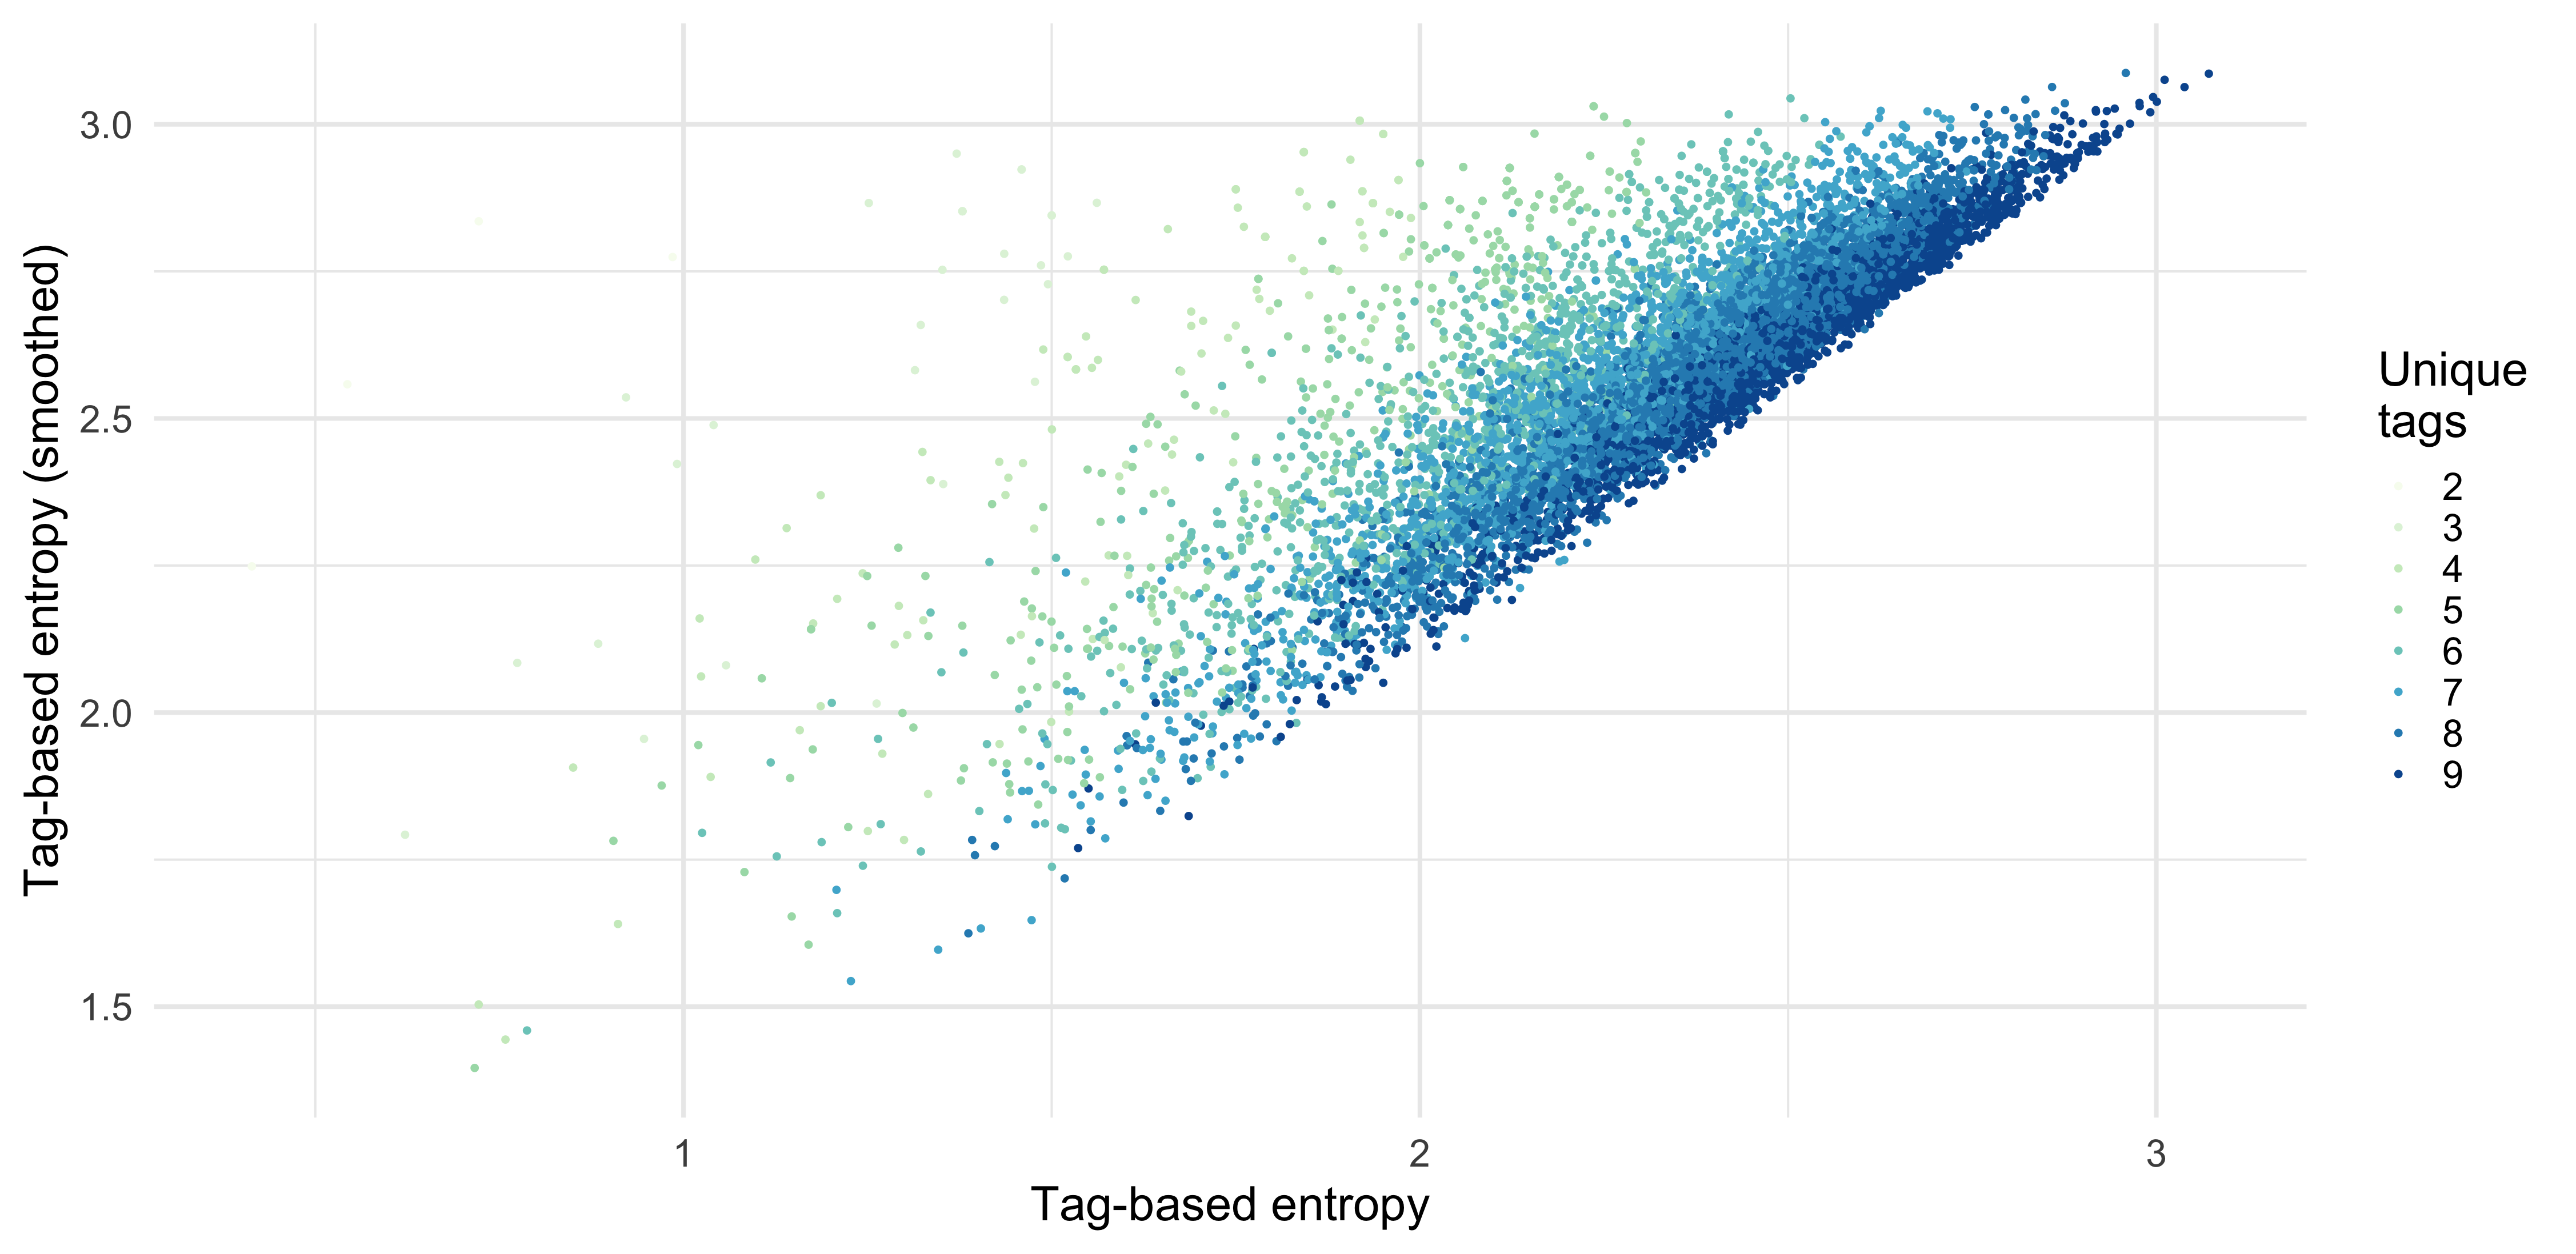
\includegraphics[width=0.9\textwidth]{\figdir/entropy_tag_vs_nunique.png}
    \end{center}
\end{figure}

